\testfile{pgfplotstest.scanline.tex}

\testsection{2D Scanline markers}
\newcommand\TEST{%
	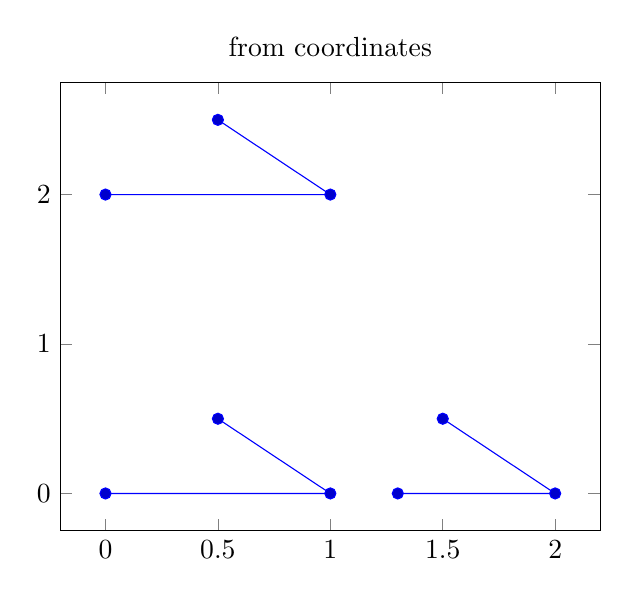
\begin{tikzpicture}
		\begin{axis}[title=from coordinates]
		\addplot coordinates {
			(0,0) (1,0) (0.5,0.5)

			(1.3,0) (2,0) (1.5,0.5)

			(0,2) (1,2) (0.5,2.5)
		};
		\end{axis}
	\end{tikzpicture}

	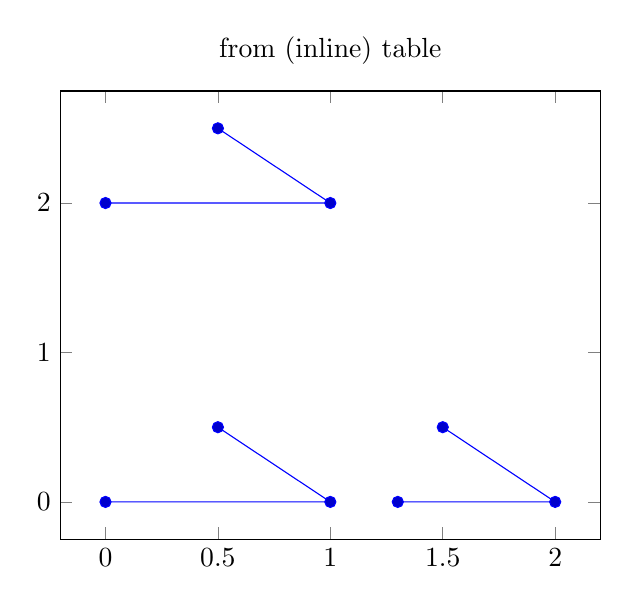
\begin{tikzpicture}
		\begin{axis}[title=from (inline) table]
		\addplot table[row sep=\\]{
			x y\\
			 0 0  \\
			 1 0 \\
			 0.5 0.5 \\
\\
			 1.3 0  \\
			 2 0  \\
			 1.5 0.5 \\
\\
			 0 2  \\
			 1 2  \\
			 0.5 2.5 \\
		};
		\end{axis}
	\end{tikzpicture}
}%
\testsubsection{empty line set to initial config (auto)}
{
	\TEST
}

\testsubsection{empty line=no op}
{
	\pgfplotsset{empty line=no op}
	\TEST
}
